\section{Prueba 1: rendimiento de módulos Linkbird-MX}
El objetivo de esta prueba es medir el rendimiento de los módulos empleados para la comunicación vehicular NEC Linkbird-MX. Se ha adaptado los programas realizados para la comunicación entre \gls{rsu} y \gls{obu} para estas pruebas mediante la integración de un módulo que registra el envío de paquetes junto con información para realizar después de las pruebas un análisis de los resultados. Para la realización se emplean dos módulos integrados en vehículos diferentes, cada vehículo tiene un rol distinto en cada test realizado:

\begin{enumerate}
	\item \textbf{Mensajes entre dos \gls{obu} en entorno urbano}: se realiza 	una ruta por la calle principal de Bilbao, donde se recogen datos en vías con una alta congestión de tráfico.
	
	\item \textbf{Mensajes entre dos \gls{obu} en vías de alta velocidad}: se realiza una ruta por la salida de la ciudad, autopista y entrada a la ciudad.
	
	\item \textbf{Mensajes entre un \gls{obu} y un \gls{rsu}}: uno de los vehículos es instalado en la carretera actuando como una \gls{rsu}, mientras el otro vehículo circula por la vía colindante alejándose y	acercándose a la unidad.
\end{enumerate}

Entre las unidades se envían mensajes de presencia, los cuales son registrados en un fichero \emph{log}. En estos ficheros se recogen datos para poder analizar la calidad de las comunicaciones entre los dos enlaces durante las pruebas realizadas. Los datos que se han deseado obtener son los siguientes: identificador del mensaje, timestamp de envío de un mensaje y timestamp de la recepción del mensaje, tamaño del mensaje y posición \gls{gps} del vehículo.

A partir de estas pruebas se deben generar estadísticas sobre el número de paquetes enviados y recibidos, en relación a la distancia entre la que se comunican los dos vehículos.

\subsection{Resultados}
Las aplicaciones funcionaron correctamente durante las pruebas y se obtuvieron los datos deseados. Tras las pruebas se generaron estadísticas como la que se puede observar en la figura \ref{fig:prueba1}, en la que se puede observar los resultados obtenidos durante la prueba en vías de alta velocidad. Los picos identificados como I, J, K y L son obtenidos durante el recorrido en la carretera,
donde existen un mayor número de obstáculos y distancia. El resto de picos identificados, han sido generados debido a una pérdida de paquetes durante curvas muy cerradas donde no hay visibilidad directa.

\begin{figure}[H]
	\begin{center}
		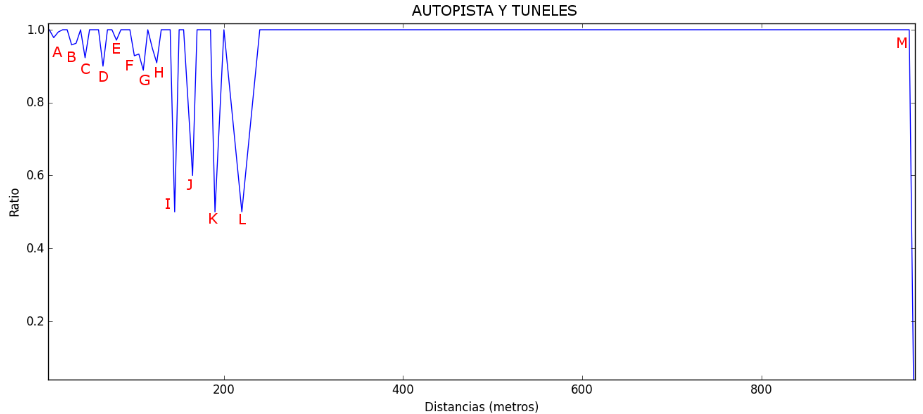
\includegraphics[scale=0.4]{prueba1-estadistica}
		\caption{Estadística Ratio/Distancia}
		\label{fig:prueba1}
	\end{center}
\end{figure}